\documentclass[final]{beamer}

% ====================
% Packages
% ====================
\usepackage[T1]{fontenc}
\usepackage{lmodern}
\usepackage[size=custom,width=120,height=73,scale=1.0]{beamerposter}
\usetheme{gemini}
\usepackage{type1cm} % Allows arbitrary font scaling
\usepackage{lmodern} % Better font rendering
\usecolortheme{gemini}
\usepackage{graphicx}
\usepackage{booktabs}
\usepackage{tikz}
\usepackage{svg} % Required for the .svg logos
\newcommand{\samelineand}{\hspace{2em}} % separates institutes on the

\usepackage{url}
\def\UrlBreaks{\do\/\do-} % Allows breaks at slashes and hyphenssame line
% ====================
% ====================
% Lengths
% ====================
% (N+1)*\sepwidth + N*\colwidth = \paperwidth
\newlength{\sepwidth}
\newlength{\colwidth}
\setlength{\sepwidth}{0.025\paperwidth}
\setlength{\colwidth}{0.3\paperwidth}
\newcommand{\separatorcolumn}{\begin{column}{\sepwidth}\end{column}}


% ====================
% Title / Author Info
% ====================
\title{Beyond Reward Maximization: Evaluating the Diversity of Trajectories in Reinforcement Learning with Temporal Vendi Score}
\author{Tom Stanic \inst{1}, Marco Jiralerspong \inst{1, 2}, Xiaofeng Zhang \inst{1, 2}, Danilo Vucetic \inst{1, 2}, Gauthier Gidel \inst{1, 2, 3}}
\institute[shortinst]{\inst{1} Université de Montréal \samelineand \inst{2} Mila -- Institut Québécois d'Intelligence Artificielle \samelineand \inst{3} CIFAR}

% ====================
% Logos 
% ====================
\logoleft{\hspace*{+2.0cm}\includesvg[height=3.2cm]{figures/mila.svg}}
\logoright{\includesvg[height=3.2cm]{figures/udem.svg}}

% ====================
% Body
% ====================
\begin{document}

\begin{frame}[t]
\begin{columns}[t]
\separatorcolumn

% ====================
% COLUMN 1
% ====================
\begin{column}{\colwidth}
  \begin{block}{Motivation}
    \begin{itemize}
      \item In reinforcement learning, an agent's task should go beyond maximizing a single scalar reward \cite{Sutton1998}; identifying diverse sets of high-quality trajectories is essential for discovering novel solutions and learning useful skills \cite{eysenbach2018diversityneedlearningskills}.
      \item Existing metrics improve exploration during training but fall short when evaluating and comparing the general diversity induced by different agents.
      \item Common proxies like state coverage or policy entropy measure properties adjacent to diversity and can be easily misled by action noise. \textbf{For instance, a policy might appear highly diverse due to random, jittery actions at each step, even if all trajectories ultimately collapse into the exact same behavioral path.}
    \end{itemize}
  \end{block}

  \begin{block}{Contributions}
    \begin{itemize}
      \item We introduce the \textbf{Temporal Vendi Score (TVS)}, a novel, domain-agnostic standard designed to measure the behavioral diversity of RL agents.
      \item TVS captures the sequential nature of state visitations and aligns with the temporal structure of the underlying Markov Decision Process (MDP) rather than relying on order-agnostic comparisons.
    \end{itemize}
  \end{block}

  \begin{alertblock}{Methodology: Temporal Vendi Score}
    Our approach evaluates diversity by assessing the variations in the induced distribution of trajectories. The computation involves three key steps:
    \begin{enumerate}
      \item \textbf{Sample Trajectories:} First, trajectories are sampled from an agent or a population of agents through environment rollouts.
      \item \textbf{Measure Similarity:} We determine the similarity between pairs of trajectories $\tau = (s_1, \dots, s_L)$ and $\tau' = (s'_1, \dots, s'_{L'})$ using the Global Alignment Kernel (GAK) \cite{cuturi2007kernel}. 
      
      \begin{equation*}
          k(\tau, \tau') = \sum_{\pi \in \mathcal{A}(\tau, \tau')} \prod_{(i, j) \in \pi} \kappa(s_i, s'_j)
      \end{equation*}
      
      \begin{itemize}
        \item Here, $\mathcal{A}(\tau, \tau')$ represents the set of all valid monotonic alignment paths between the two trajectories, and $s_i, s'_j \in \mathcal{S}$ are the individual states at given timesteps.
        \item By marginalizing over all valid alignments $\pi$, the GAK allows us to account for sequential structure rather than just order-agnostic state visitation.
        \item To capture the environment's true geometry, the local similarity $\kappa(s_i, s'_j)$ uses a \emph{time-to-reach} distance, representing the minimum number of actions needed to transition between states.
      \end{itemize}
      \item \textbf{Aggregate Diversity:} We construct a pairwise similarity matrix and compute its eigenvalues using the Vendi score \cite{friedman2023vendiscorediversityevaluation}. This yields a single, interpretable scalar value representing general population diversity.
    \end{enumerate}
  \end{alertblock}
\end{column}

\separatorcolumn

% ====================
% COLUMN 2
% ====================
\begin{column}{\colwidth}
  % Methodology Figure at the top of Column 2
  \begin{figure}
    \centering
    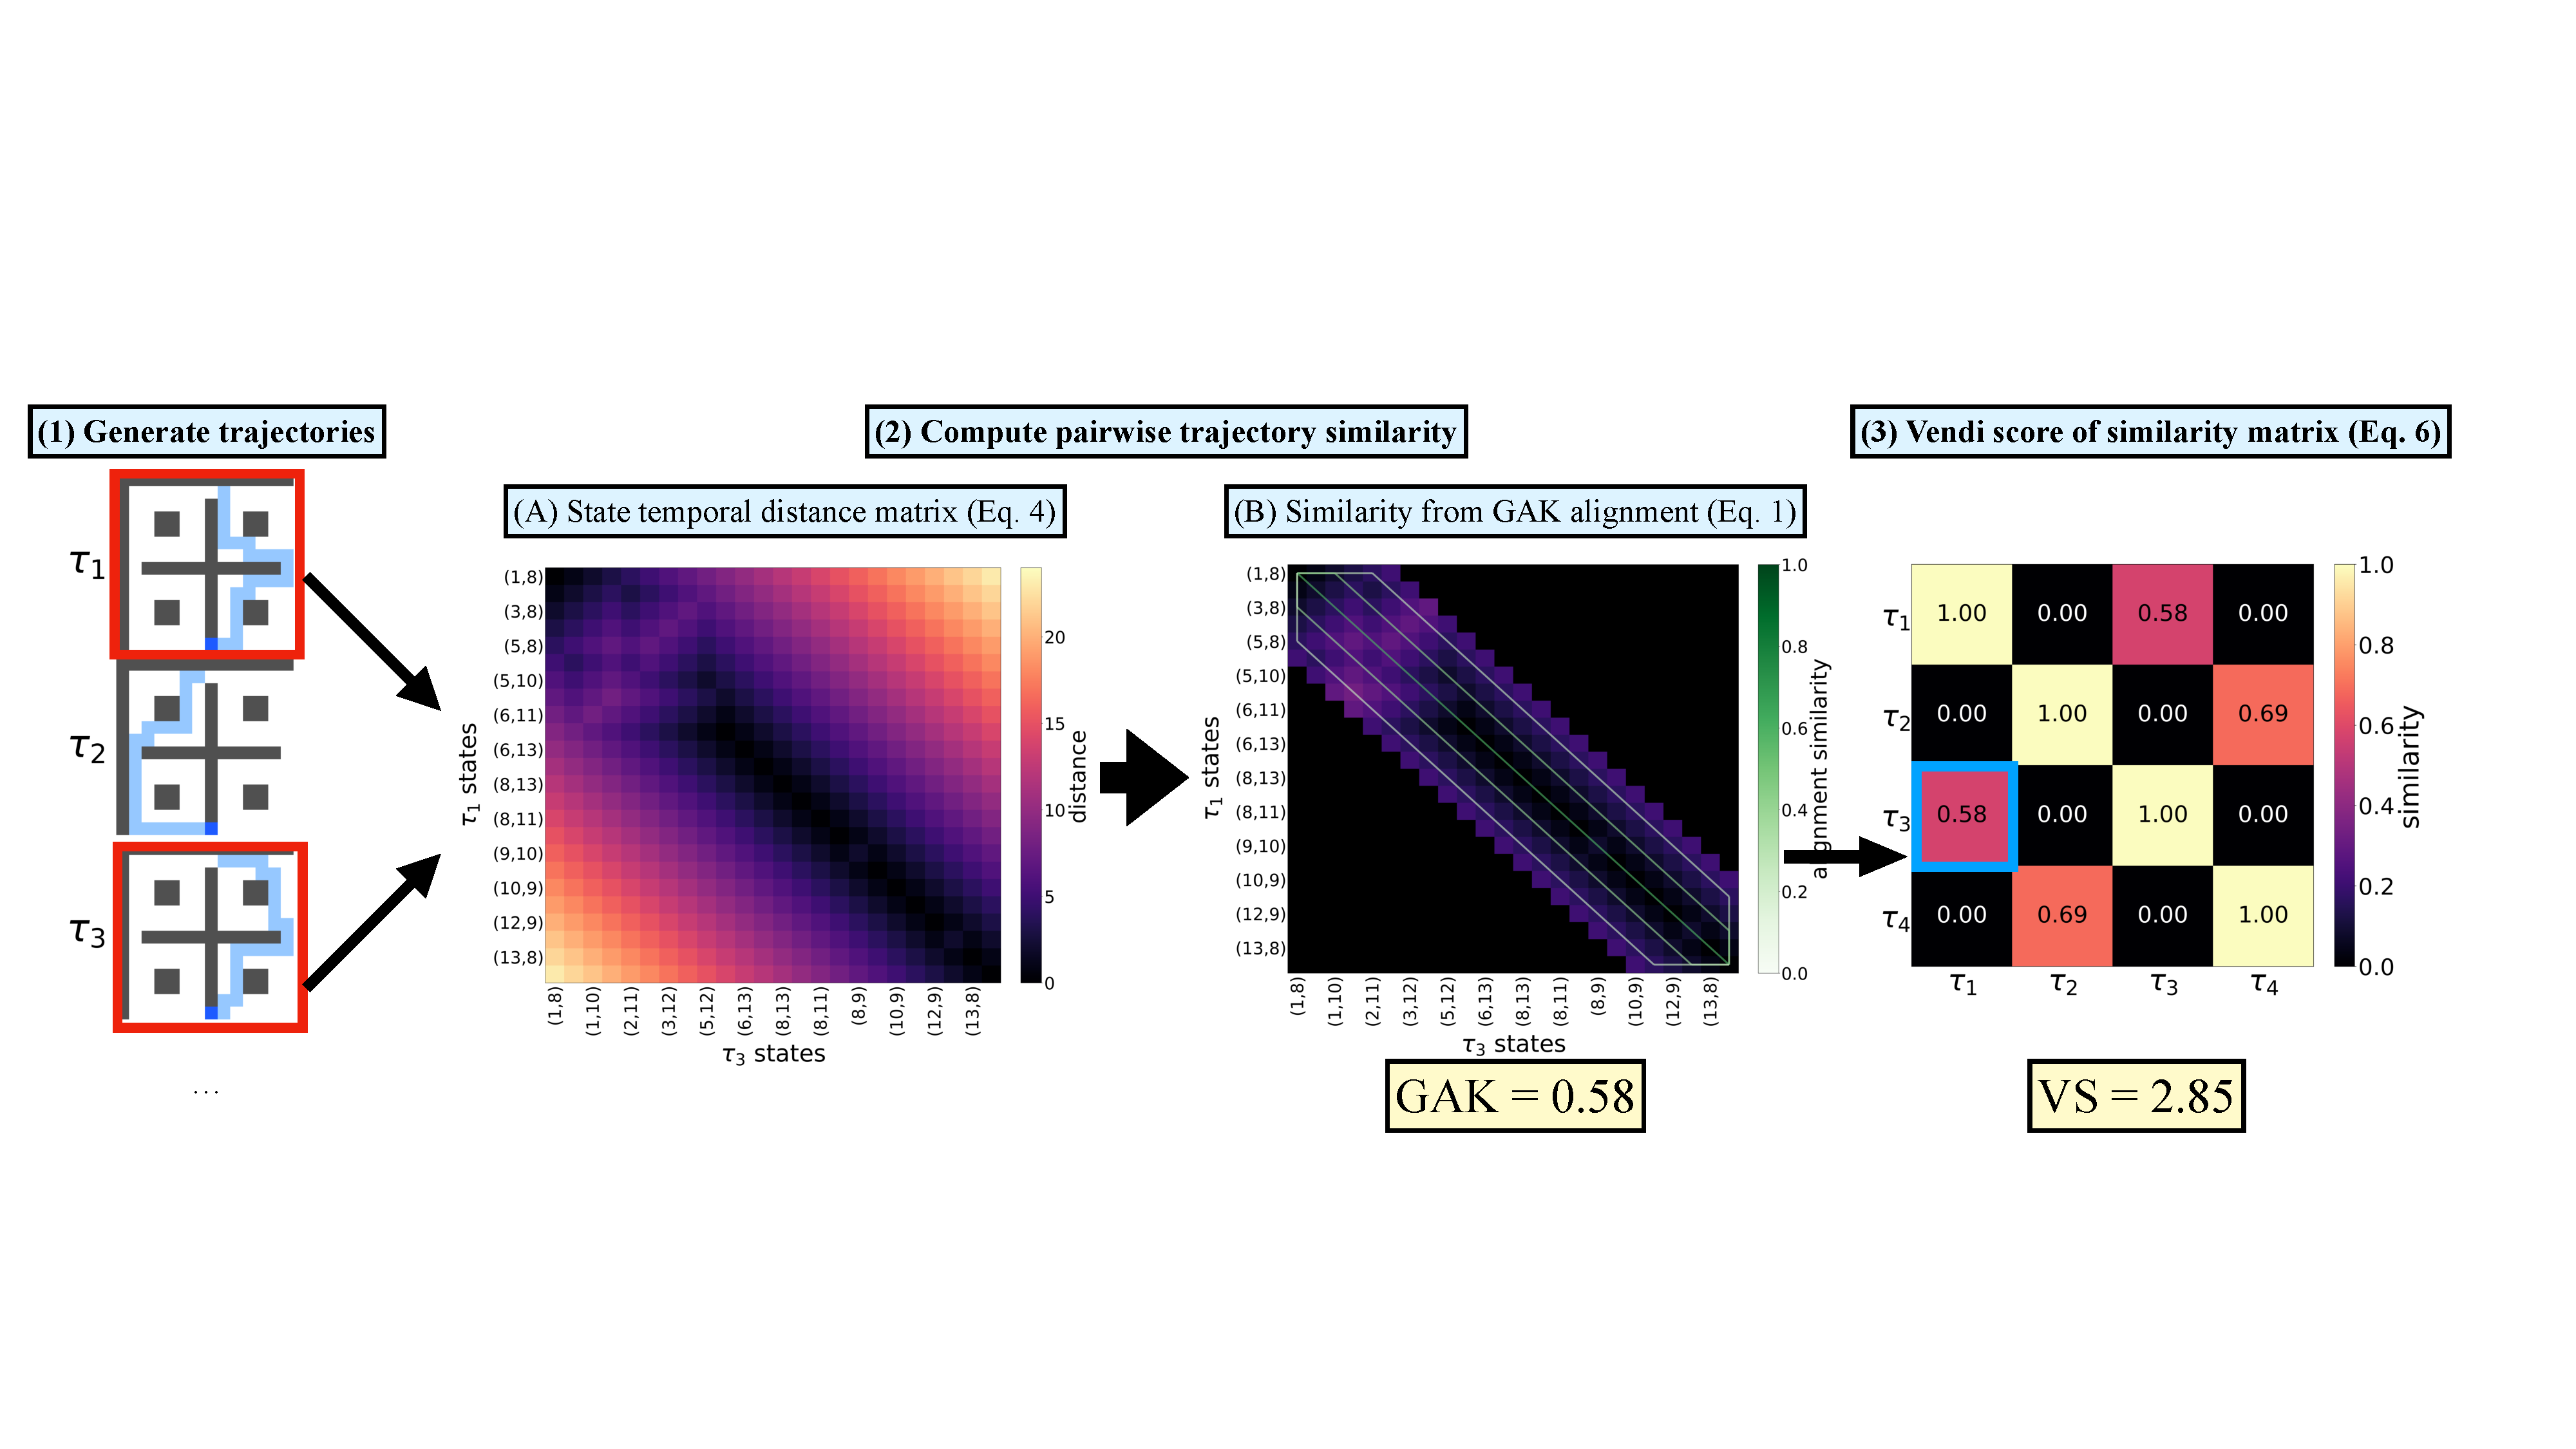
\includegraphics[width=0.95\linewidth]{figures/method.pdf}
    \caption{Procedure for computing the Temporal Vendi Score (TVS). (1) Trajectories are sampled from the agent. (2A) For each pair of trajectories, a pairwise state temporal distance matrix is computed whose entries correspond to the symmetrized time-to-reach distance between a pair of states $s_i, s'_j$. (2B) A truncated band of this matrix is used to compute the GAK alignment. The resulting GAK is used as a similarity value between that pair of trajectories. (3) TVS is computed from the eigenvalues of the resulting pairwise similarity matrix.}
    \label{fig:method}
  \end{figure}

  \begin{block}{Experiments \& Key Results}
    \begin{itemize}
      \item \textbf{Interpretability:} In grid mazes with verifiable diversity, TVS successfully produces scores that tightly correlate with the actual number of distinct behavioral strategies (see Figure~\ref{fig:interpretability}).
    \end{itemize}
    
    \begin{figure}
        \centering
        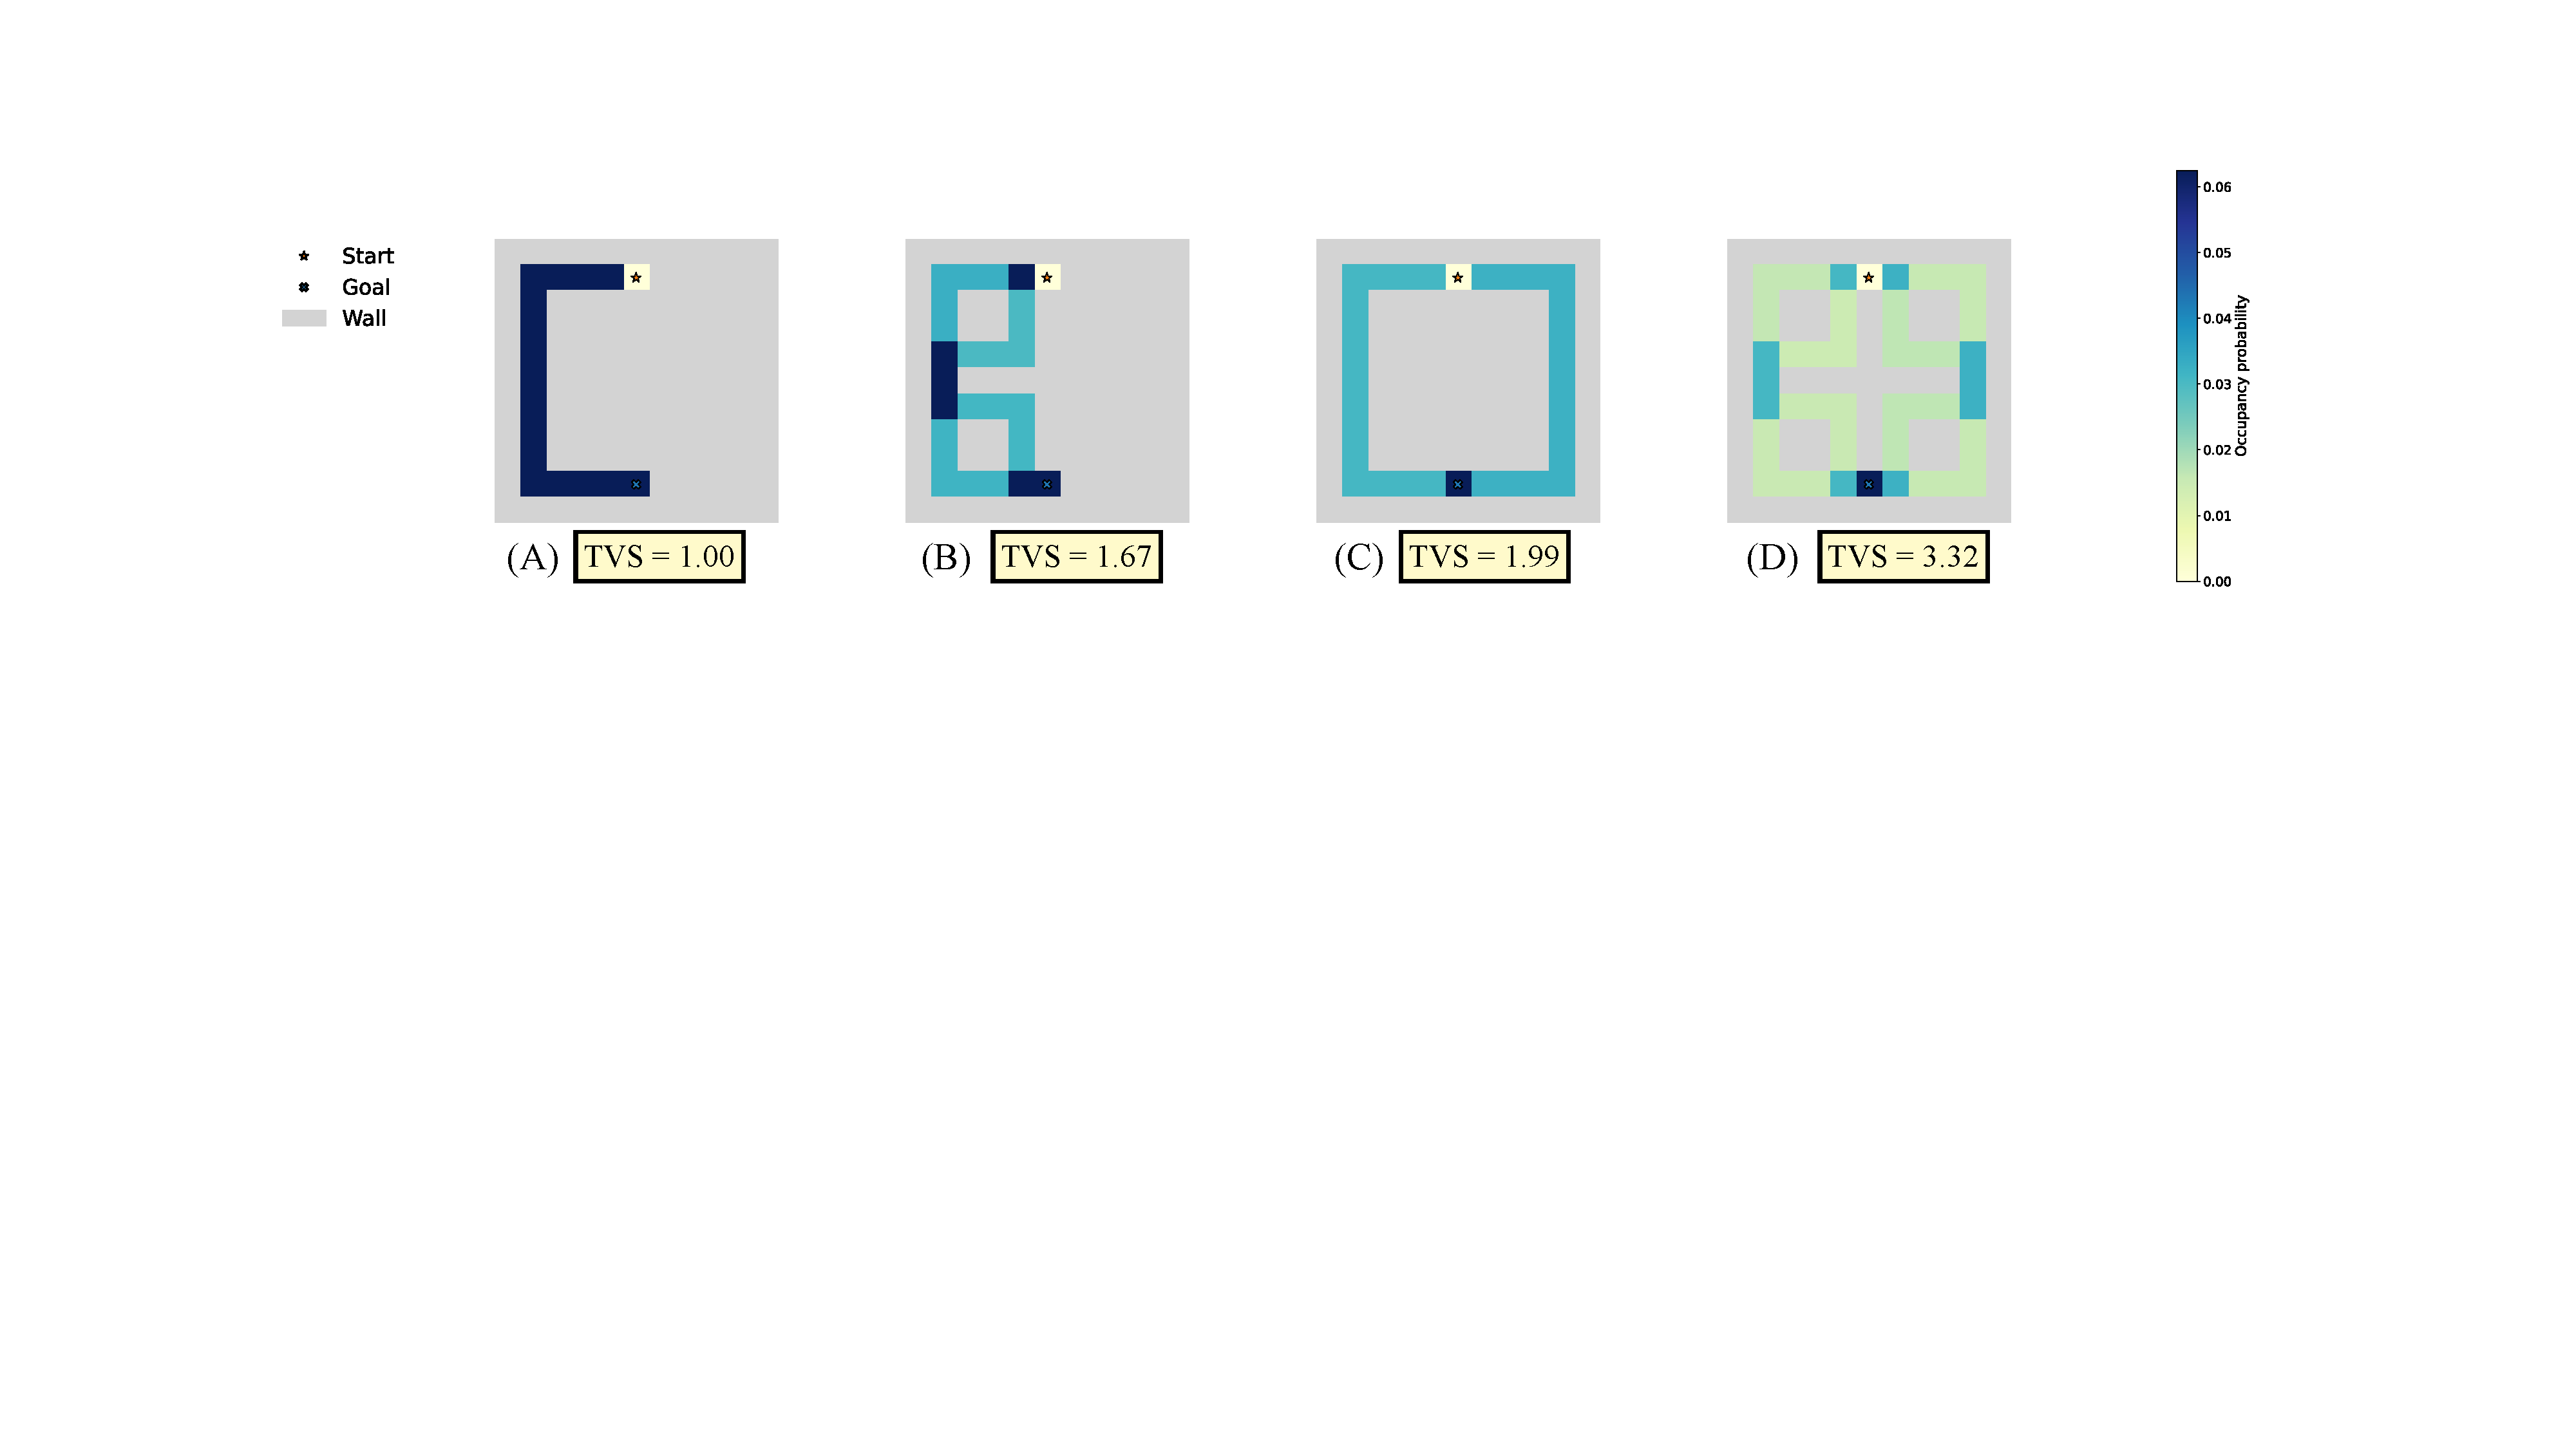
\includegraphics[width=0.85\linewidth]{figures/interpretable.pdf}
        \caption{TVS of agents with increasing diversity in a simple grid maze. The maze admits paths on both its left and right sides. (A) Single path to the goal. (B) Four overlapping paths on the left. (C) Two distinct paths, one on each side. (D) Eight overlapping paths, mirroring (B) on both sides.}
        \label{fig:interpretability}
    \end{figure}
  \end{block}
\end{column}

\separatorcolumn

% ====================
% COLUMN 3
% ====================
\begin{column}{\colwidth}
  \begin{block}{Experiments \& Key Results (continued)}
    \begin{itemize}
      \item \textbf{Superiority Over Baselines:} When agents learn to solve a task using temporally diverse sequences (e.g., using different keys in different orders), state-level metrics like state coverage and occupancy entropy remain completely flat. In contrast, TVS effectively captures this sequential structure and scales properly as agents learn new strategies (see Figure~\ref{fig:key_baseline}).
      
        \begin{figure}
            \centering
            % Ensure this filename matches your actual key environment plot
            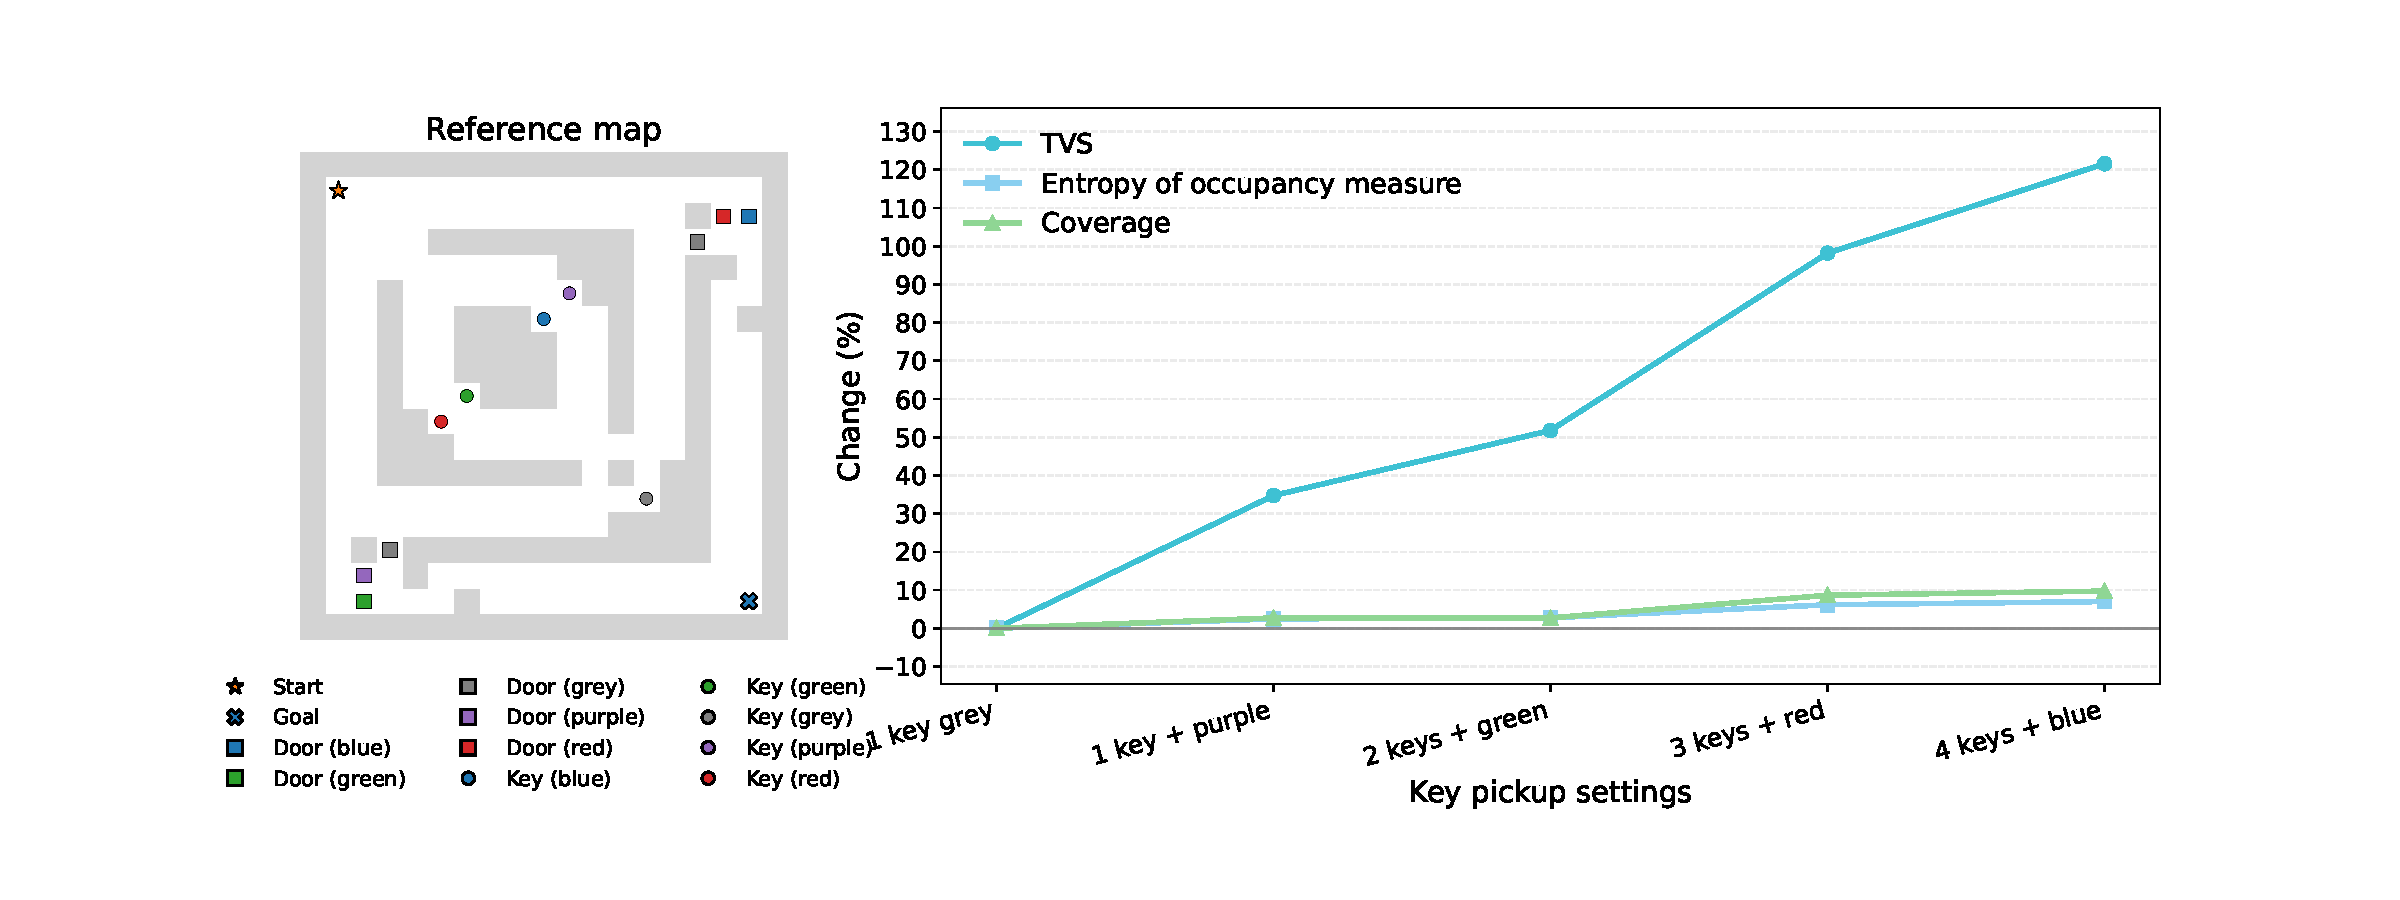
\includegraphics[width=0.85\linewidth]{figures/key.pdf} 
            \caption{Comparison of TVS against state-level baselines in a sequential key-gathering environment.}
            \label{fig:key_baseline}
        \end{figure}

      \item \textbf{Sample Efficiency:} Extensive evaluations indicate that TVS converges to a stable and reliable score with a modest number of samples \cite{pasarkar2024cousinsvendiscorefamily}, requiring approximately 128 rollouts across various environment sizes, and scales effectively to evaluate agents in continuous control settings (see Figure~\ref{fig:sample_efficiency}).
      
        \begin{figure}
            \centering
            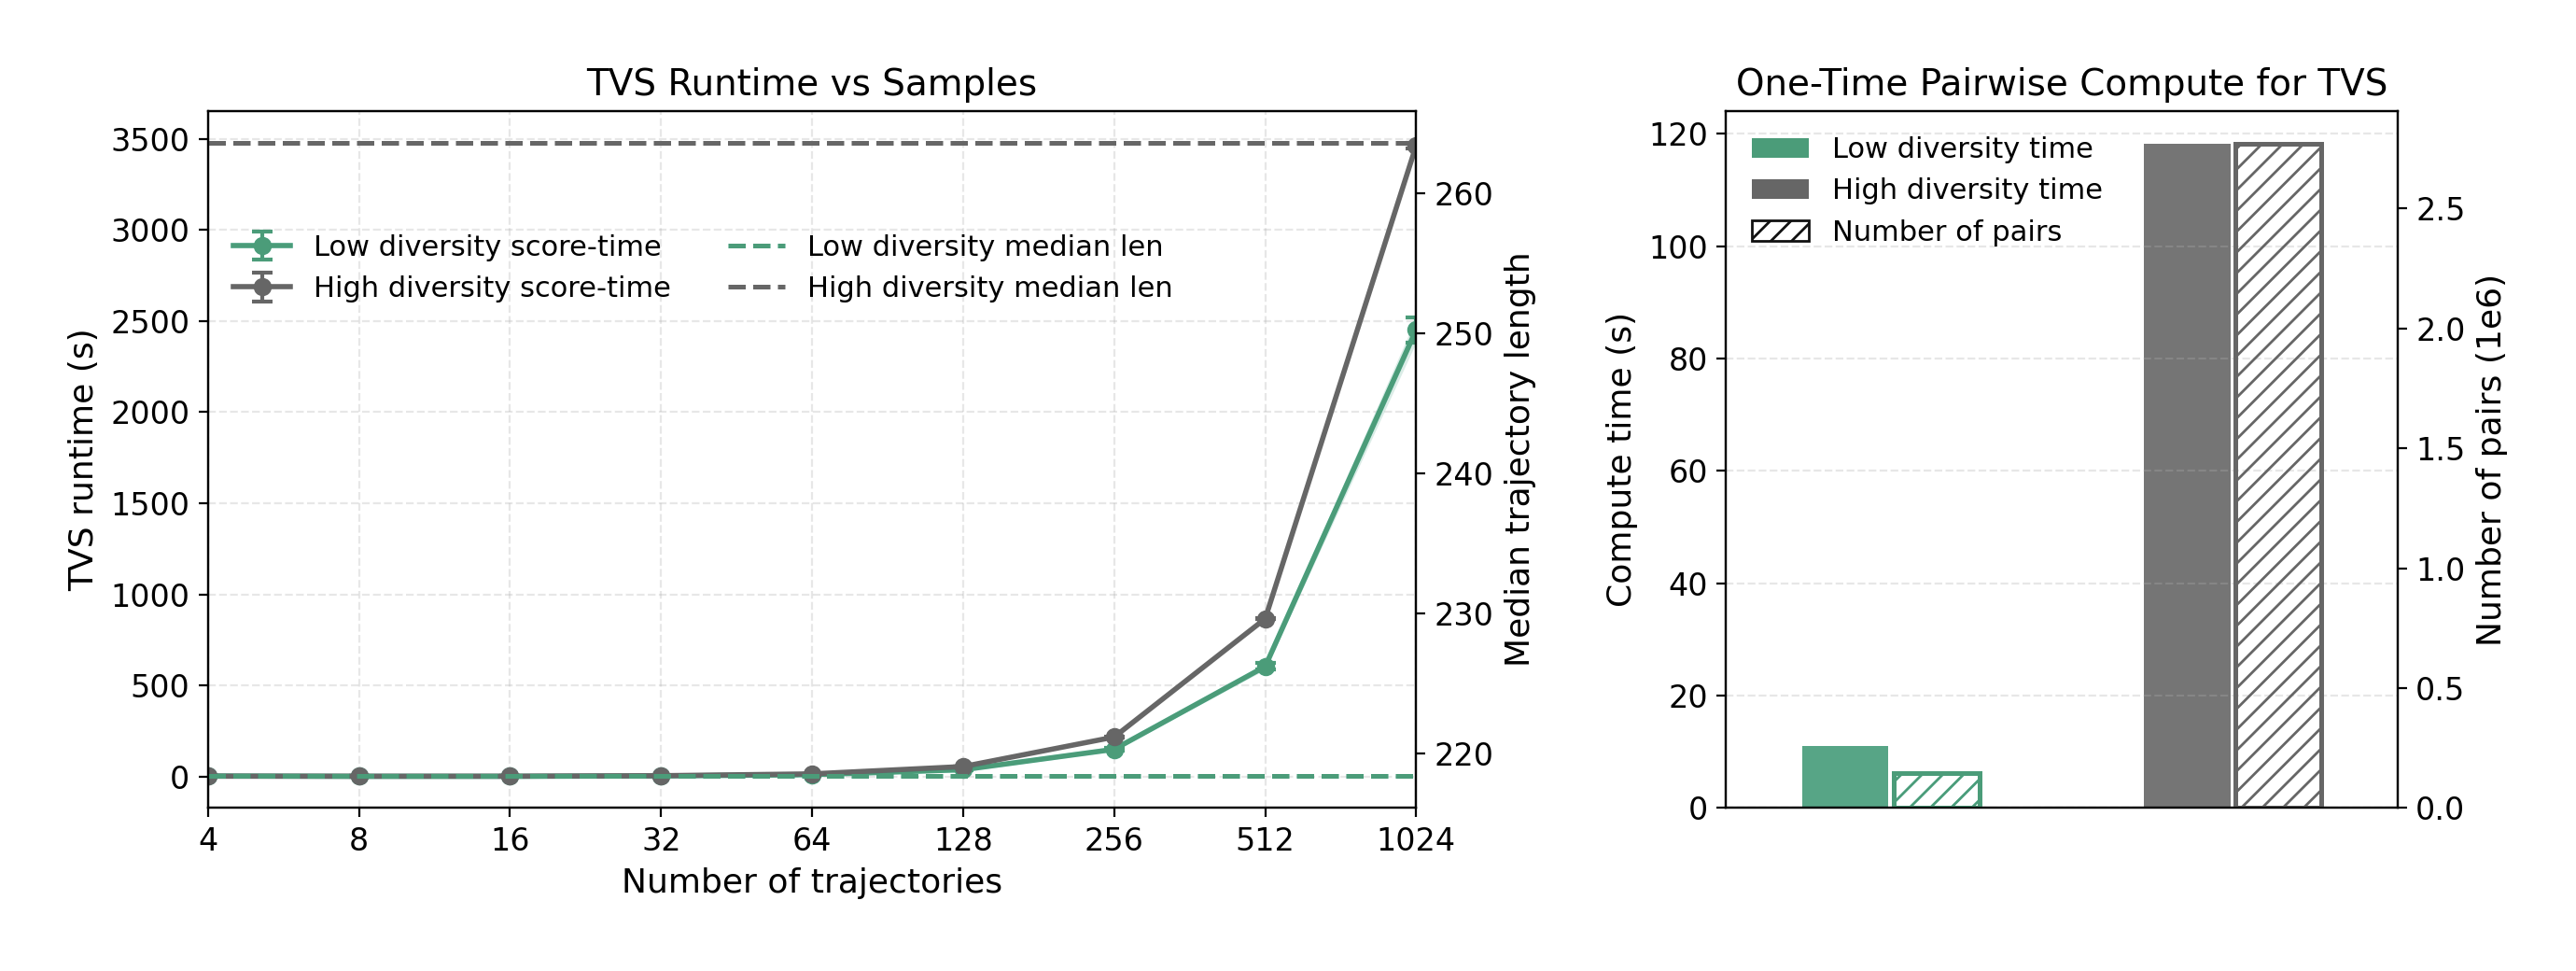
\includegraphics[width=0.85\linewidth]{figures/vendi_time_1024.png}
            \caption{Computation cost and sample efficiency of TVS in a continuous point maze environment.}
            \label{fig:sample_efficiency}
        \end{figure}
    \end{itemize}
  \end{block}

  \begin{block}{References}
    \footnotesize % Reduces font size for references to save space
    \bibliographystyle{plain}
    % Ensure your bib file is in the same directory and named properly
    \bibliography{poster}
  \end{block}
\end{column}

\separatorcolumn
\end{columns}
\end{frame}

\end{document}